\documentclass[a4paper, 11pt, normalem]{report}

\usepackage{../../../LaTeX-Templates/Notes}

\titlecontents{chapter}% <section-type>
    [0pt]% <left>
    {}% <above-code>
    {Lecture \thecontentslabel\quad}% <numbered-entry-format>
    {}% <numberless-entry-format>
    {\dotfill\contentspage}% <filler-page-format>
\titleformat{\chapter}{\fontsize{15}{17}\bfseries\normalfont}{\textbf{Lecture \thechapter}}{1em}{}
\titleformat{\subsubsection}{\fontsize{10}{13}\bfseries\scshape}{\textbf{\thesubsubsection}}{1em}{}
\setcounter{tocdepth}{4}
% \setcounter{secnumdepth}{1}

\renewcommand{\arraystretch}{1.2}

\newcommand\p{\partial}
\newcommand\E{\mathcal{E}}
\newcommand\uE{\unl{\E}}
\newcommand\B{\mathcal{B}}
\newcommand\uB{\unl{\B}}
\newcommand\del{\unl{\nabla}}
\newcommand\eno{\epsilon_0}
\newcommand\hi{\hat{i}}
\newcommand\hj{\hat{j}}
\newcommand\hk{\hat{k}}
\newcommand\hn{\hat{n}}

\title{Foundations of Physics 2A \\ Electromagnetism \vspace{-20pt}}
\author{Professor D P Hampshire}
\date{\vspace{-15pt}Epiphany Term 2018}
\rhead{\hyperlink{page.1}{Go to TOC}}

% \begin{example}[Title]
%
% \end{example}

\begin{document}

\maketitle
\tableofcontents

\chapter{}

\section{Maxwell's Equations and Classical Physics}
Feynman claims that there are seven equations that describe all of classical physics; the first four of these are Maxwell's Equations:
\begin{enumerate}
    \item From Coulomb's Law:
        \begin{equation}
            \del\cdot\uE = \frac{\rho}{\epsilon_0} \tag{M\RN{1}}
        \end{equation}
    \item Given no magnetic monopoles have been observed:
        \begin{equation}
            \del\cdot \uB = 0 \tag{M\RN{2}}
        \end{equation}
    \item From Faraday's Law of Induction:
        \begin{equation}
            \del \times \uE = -\frac{\p \B}{\p t} \tag{M\RN{3}}
        \end{equation}
    \item From Ampere's Law:
        \begin{equation}
            \del \times \uB = \mu_0 \unl{J} + \mu_0 \eno \frac{\p \E}{\p t} \tag{M\RN{4}}
        \end{equation}
        where the symbol $\del$ denotes the vector operator 'del':
        \begin{equation*}
            \del = \hi \frac{\p}{\p x} + \hj \frac{\p}{\p y} + \hk \frac{\p}{\p z}
        \end{equation*}
        \begin{itemize}
            \item $\uE$ - electric field ($V\,m^{-1}$)
            \item $\uB$ - magnetic field ($T$)
            \item $\rho$ - total charge density ($C\,m^{-3}$)
            \item $\unl{J}$ - total current density ($A\,m^{-2}$)
        \end{itemize}
    \item Force on a moving charge in a magnetic and electric field:
        \begin{equation*}
            \unl{F} = q(\uE + \unl{v} \times \uB)
        \end{equation*}
    \item Newton's Law of Motion:
        \begin{equation*}
            \unl{F} = \frac{d\unl{p}}{dt}, ~ \unl{p} = \frac{m\unl{v}}{\sqrt{1 - \frac{v^2}{c^2}}}
        \end{equation*}
    \item Newton's Law of Gravity:
        \begin{equation*}
            \unl{F} = -\frac{Gm_1 m_2}{r^2}\hat{r}_{1 \to 2}
        \end{equation*}
\end{enumerate}

\subsection{General Comments}
\begin{itemize}
    \item There is no agreed order for Maxwell's equations.
    \item Maxwell's equations are completely general and valid at every point in space and time.
    \item There is a divergence equation (i.e. $\del \cdot$) for both $\uE$ and $\uB$ and a curl equation (i.e. $\del \times$) for each as well.
    \item $\uE$ and $\uB$ always refer to the net field.
\end{itemize}

\section{Maxwell's Equations and Vector Fields}
\subsection{The Flux of a Vector Field}
A vector field is fully characterised by knowing its magnitude and direction at every point in space and time.

An arbitrarily shaped three-dimensional 'closed surface' is the surface of the volume. \\
A smooth 'open surface' is also shown which does not enclose volume and has edges.
\begin{equation*}
    d\unl{S} = \hn \cdot dS
\end{equation*}
The vector $\hn$ is the outward normal unit vector to the surface and $\unl{h}$ is an arbitrary vector field.

By definition, the surface area element, $d\unl{S}$, is $d\unl{S} = \hn \cdot dS$, where dS is the scalar area of the element.
In general, we can say "the flux of a vector $\unl{h}$ through the surface is
\begin{equation*}
    \phi = \int \unl{h} \cdot \hn dS = \int \unl{h} \cdot d\unl{S}."
\end{equation*}

\subsubsection{Comments}
\begin{itemize}
    \item The flux of charge density is current.
    \item Flux is a useful concept for describing conservation laws - energy, momentum, charge, etc.
\end{itemize}
\emph{Be careful the joys of the English word 'density'}:
\begin{itemize}
    \item Mass density - $kg\,m^{-3}$
    \item Current density - $A\,m^{-2}$
\end{itemize}

\subsection{The Divergence Theorem}
The divergence theorem is a vector calculus identity:
\begin{equation*}
    \int \unl{h}\cdot d\unl{S} = \int \del \cdot \unl{h}dV
\end{equation*}
where $\unl{h}$ is any arbitrary vector field.

\subsection{Stoke's Theorem}
\begin{equation*}
    \int \unl{h}\cdot d\unl{l} = \int (\del \times \unl{h}) \cdot d\unl{S}
\end{equation*}
Note that $\unl{l}$ and $\unl{S}$ are vectors, V is scalar.
\begin{itemize}
    \item Divergence theorem: volume integral to surface integral
    \item Stoke's theorem: surface integral to line integral
\end{itemize}

\subsection{Vector Identities}
\begin{align*}
    \del \times (\del \times \unl{A}) &= \del(\del \cdot \unl{A}) - \nabla^2 \unl{A} \\
    \del \cdot (\unl{A} \times \unl{B}) &= \unl{B}\cdot(\del \times \unl{A}) - \unl{A} \cdot (\del \times \unl{B})
\end{align*}

\chapter{}
\section{Maxwell \RN{1}}
\subsection{Deriving Gauss' law and Maxwell \RN{1} from Coulomb's Law}
\begin{wrapfigure}{r}{0.4\textwidth}
    \begin{center}
        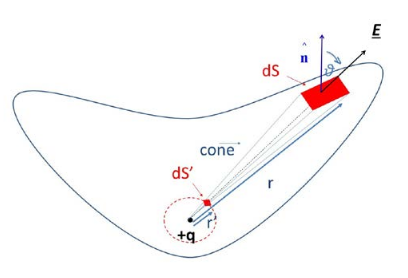
\includegraphics[scale=0.4]{fluxvec.png}
    \end{center}
\end{wrapfigure}
The cone first passes through a sphere centred about the charge and then through the surface of the arbitrary closed shape.

Consider first the sphere: \\
The electric field, $E(r')$, has constant magnitude over the surface of the sphere and is everywhere parallel to $d\unl{S}'$, i.e. $\hn\,dS'$ so we have:
\begin{equation*}
    \int \uE(r') \cdot d\unl{S}' = \frac{q}{4\pi\eno(r')^2}\cdot 4\pi(r')^2 = \frac{q}{\eno}
\end{equation*}
Consider now the flux through the elemental area $dS$, which is part of the surface of the arbitrary shape surrounding the charge.
We have:
\begin{equation*}
    \uE(\unl{r})\cdot \hn\;dS = |E(r)||\hn||\cos\theta|dS
\end{equation*}
Since $dS$ is a projection of $dS'$ (because they are both bound by the same cone), we can relate the two of them using:
\begin{equation*}
    \frac{dS'}{\pi(r')^2} = \frac{dS}{\pi r^2}\cos\theta
\end{equation*}
Substituting, we have:
\begin{align*}
    \uE(r)\cdot\hn\;dS &= E(r)\frac{r^2}{(r')^2}dS' \\
    &= \frac{q}{4\pi\eno r^2}\frac{r^2}{(r')^2} dS' \\
    &= \frac{q}{4\pi\eno(r')^2}dS'
\end{align*}
Hence the flux through the surface $dS$ is the same as the flux through $dS'$. \\
Integrating gives:
\begin{equation*}
    \int \uE\cdot d\unl{S} = \frac{q}{\eno}
\end{equation*}
Applying superposition to a collection of charges inside the arbitrary shape gives:
\begin{equation}
    \int \uE\cdot d\unl{S} = \frac{\sum q}{\eno} = \frac{1}{\eno}\int \rho\;dV \tag{Gauss' Law}
\end{equation}
Where $\rho$ is the charge density and then we can use the divergence theorem:
\begin{equation*}
    \int \del \cdot \uE dV = \frac{1}{\eno} \int \rho\;dV
\end{equation*}
Since the volume integrals are equal for any arbitrary volume, the integrands must also be equal so:
\begin{equation*}
    \del \cdot \uE = \frac{\rho}{\eno} \tag{M\RN{1}}
\end{equation*}
We conclude that Maxwell's 1st equation is a differential form of Gauss' Law, which in turn is a form of Coulomb's Law. \\
Coulomb's Law (or equivalently Gauss' Law) is only true under static conditions.
Just as with Hooke's Law, experimentation shows us that M\RN{1} is true under all conditions.

The $\uE$-field resulting from any charge distribution gives $\del \cdot \uE = 0$ in the local regions where there is no charge.














































































\end{document}
